\begin{center}
\fbox{\fbox{\parbox{6.5in}{\centering
\begin{flushleft}

\vspace{5mm}
\hspace{5mm} \textbf{\underline{Märgireeglid liitmisel/lahutamisel:} \hspace{15mm} \underline{Märgireeglid korrutamisel/jagamisel:}}\\
\vspace{2mm}
\hspace{5mm} \fbox{\parbox{1.5in}{\centering
$+(a) = +a$\\ $-(a) = -a$\\ $+(-a) = -a$\\ $-(-a) = +a$}} \hspace{5cm} \fbox{\parbox{1.5in}{\centering $(1)\cdot (1) = +1$\\ $(1)\cdot (-1) = -1$\\ $(-1)\cdot(1) = -1$\\ $(-1)\cdot (-1) = +1$}}\\
\vspace{5mm}
\hspace{5mm} \textbf{Näited:}\\
\vspace{5mm}
\hspace{5mm} a) $ -10 -(-5) +(-2) = -10 + 5 -2 = -7$\\
\vspace{2mm}
\hspace{5mm} b) $ -2\cdot (-3)+(-6)= 2\cdot 3 - 6 = 6 - 6 = 0$\\
\vspace{5mm}
\hspace{5mm} \textbf{Miinusmärk sulu ees, muudab märgid sulu sees!}\\
\vspace{5mm}
\hspace{5mm} Näiteks kui me peame suurele negatiivsele arvule liitma juurde väikese positiivse arvu (ning me\\
\hspace{5mm} ei tea kuidas seda arvutada), siis saame tõsta tehte ette miinusmärgi. See muudab tehtes \\
\hspace{5mm} kõik märgid \underline{vastupidiseks}.\\
\vspace{2mm}
\hspace{5mm} NT: $-12 + 6 = - (12 - 6) = - ( 6) = -6 $\\
\vspace{5mm}
\hspace{5mm} \textbf{\underline{Absoluutväärtus:}}\\
\vspace{5mm}
\hspace{5mm} Arvu absoluutväärtust võib pidada arvu kauguseks nullist.\\
\vspace{5mm}
\hspace{5mm} 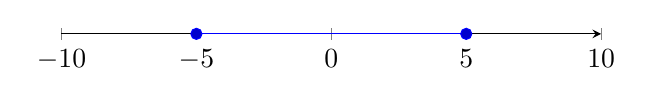
\begin{tikzpicture}
        \begin{axis}[
            % center the x axis
            axis x line=middle,
            % we don't need a y axis line ...
            axis y line=none,
            % ... and thus there is no need for much `height' of the axis
            height=50pt,
            % but `height' also changes `width' which is restored here
            width=\axisdefaultwidth,
            xmin=-10,
            xmax=10,]
            \addplot coordinates {(5,0) (-5,0)};
        \end{axis}
    \end{tikzpicture}\\
\vspace{2mm}
\hspace{5mm} Nagu näha (loodetavasti, kui paber on värviline), siis arvtelje punktid koordinaatidega ($-5$) ning (5)\\ \hspace{5mm} asuvad nullpunktist ühesugusel kaugusel. Samuti peaks see olema ilmselge, et tegelikult ei saa meil olla\\ \hspace{5mm}  ''negatiivseid'' kauguseid. Keegi ei saa olla ''miinus 1 ja pool meetrit pikk''. Nii, et kuna absoluutväärtus\\ \hspace{5mm} väidabki, et tegemist on \underline{kaugusega} nullpunktist, siis peab see suurus olema positiivne, sõltumata\\ \hspace{5mm} sellest, kummal pool arvtelge see arv asub.\\
\vspace{5mm}
\hspace{5mm} \textbf{Näiteks:}
\vspace{5mm}

\hspace{5mm} a) $|-5| + 5 = 5 + 5 = 10$\\
\vspace{2mm}
\hspace{5mm} b) $|5| + |-5| = 5 + 5 = 10$,\hspace{1cm}  kuna $|-5|$ kui ka $|5|$ mõlemad võrduvad (+5)-ga.\\
\vspace{2mm}
\hspace{5mm} c) $-1\cdot 10 + |-10| = -10 + 10 = 0$\\
\vspace{5mm}
\end{flushleft} }}}
\end{center}

\newpage


\begin{center}
\fbox{\fbox{\parbox{6.5in}{\centering
\begin{flushleft}
\hspace{5mm} \textbf{\underline{Korduvate arvude kirjutamine korrutise abil}}\\
\vspace{5mm}
\hspace{5mm} Kui mingis tehtes peaksid meil arvud (liidetavad või lahutatavad)  korduma, siis neid saab palju\\ \hspace{5mm} lühemalt kirja panna korrutise  kujul. 

\vspace{2mm}
\hspace{5mm}
\textbf{Näiteks:}\\
\vspace{5mm}
\hspace{5mm} a) $10+5+5+5 = 10 + 5\cdot 3$ \hspace{5mm} sest arv ''5'' kordub meil 3 korda.\\
\vspace{5mm}
\hspace{5mm} b) $9-(-5)-(-5)-(-5)= 9 - [(-5) \cdot 3] = 9 + 5 \cdot 3 = 9 + 15$ \hspace{5mm} sest arv ''$-5$'' kordub meil 3 korda.\\
\vspace{5mm}
\hspace{5mm} \textbf{\underline{Tehetejärjekord:}} \hspace{5mm} $Sulud \rightarrow astmed \rightarrow korrutamine/jagamine \rightarrow liitmine/lahutamine.$
\end{flushleft} }}}
\end{center}

\vspace{1cm}

\textbf{Märkmed}\\
\vspace{2mm}
\begin{mdframed}[style=graphpaper]
\vspace{14cm}
\end{mdframed}